\documentclass[10pt,letterpaper,english]{article}

\usepackage{graphicx}
\usepackage{wrapfig}

\pagestyle{empty}


\setlength{\oddsidemargin}{0in}
\setlength{\evensidemargin}{0in}
\addtolength{\textwidth}{1in}
\addtolength{\topmargin}{-.25in}
\addtolength{\textheight}{.5in}

\begin{document}

\newcommand\generatepages{\input{TEXT.tex}}

\newcommand{\handout}[2]{
\newpage
\subsection*{Broken Telephone Tree}

\begin{centering}
\fbox{
\parbox{\textwidth}
{{\em Broken Telephone is a game in which each successive participant secretly whispers to the next a phrase or sentence whispered to them by the preceding participant. Cumulative errors from mishearing often result in the sentence heard by the last player differing greatly and amusingly from the one uttered by the first... It is often invoked as a metaphor for cumulative error, especially the inaccuracies of rumours or gossip.} \hspace*{\fill} (Wikipedia)}
}
\end{centering}

In this class, we will {\bf not} be playing Broken Telephone, {\em per se}.
Instead, we will be assuming that we have just walked in on a room where
it has been played.
We are given the final version(s) of the message
and it is our job to reconstruct the original.
We are therefore analyzing the {\em output} of a broken telephone network,
rather than simulating the broken telephone itself.

The game that was played here, whose output we will analyze, is slightly different
to the classical version (see Wikipedia description, above).
In our version, the message network was not a linear
chain of participants, but rather a {\em telephone tree}
(a typical communications tool
 of neighborhood watch groups, parent-teacher associations,
 and clandestine spy networks).

\begin{wrapfigure}[8]{r}{.2\textwidth}
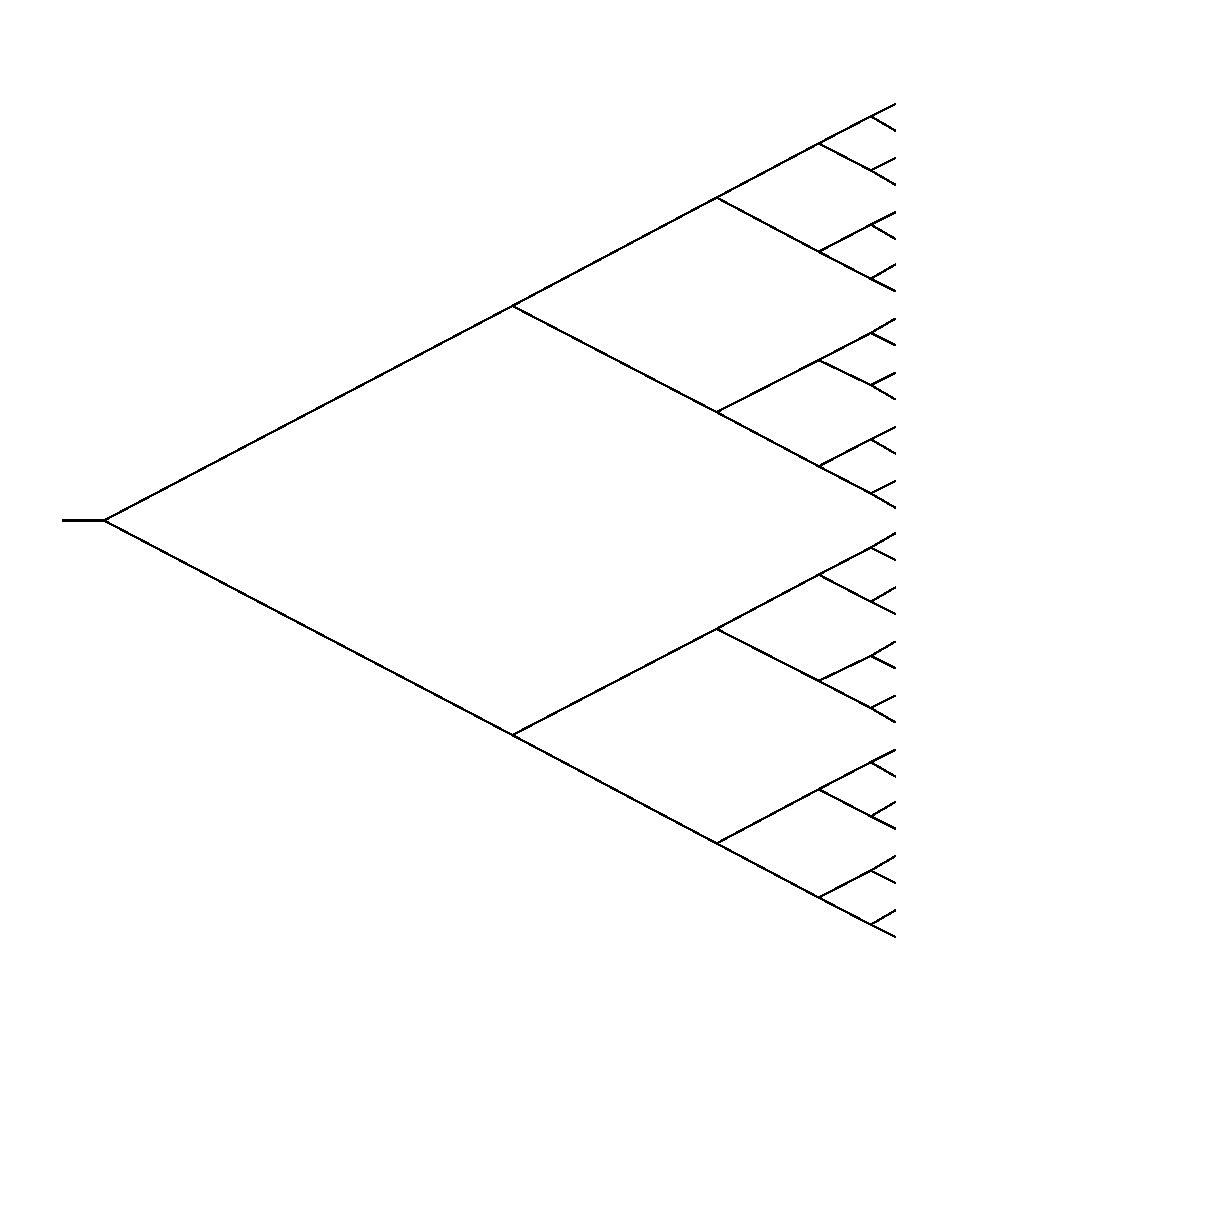
\includegraphics[width=.2\textwidth,trim=0 1in 2in 1in]{tree32.pdf}
\end{wrapfigure}

In our {\em broken telephone tree}, each participant whispers the message twice.
(By ``whispering'' we mean transmitting the message with a few errors.)
The first person whispers their message to two people, those two people each whisper their version of the message to four more people, and so on: the number of messages doubles at every round.
The process continues for five rounds, after which there are $2^5=32$ different final versions of the message (plus 31=1+2+4+8+16 intermediate versions).
Thus, the phone network is a {\em bifurcating tree} with 32 {\em leaf nodes}, as shown to the right.

There are 63 agents---of whom 31 are intermediate message couriers, and the remaining 32 are final message recipients---whose relationships we'd like to reconstruct.
We can't interrogate the agents directly,
so we seek to understand the network using available signals intelligence.

Our intercepts are limited to the final 32 versions of the message.
We don't have the 31 intermediate messages,
nor do we know who called whom (i.e. the structure of the telephone tree) beyond the fact that it was a bifurcating tree.
Only the 32 final messages remain; in fact, the piece of paper you're holding includes only one of those messages.

Your goal, and the real point of this version of the game, is to reconstruct as much as possible of the {\bf original} message --- {\em and} the structure of the transmission network.
The problem is directly analogous to reconstructing the evolutionary history ({\bf phylogeny} and {\bf alignment}) of DNA, RNA, and protein sequences found in genomes.

{\bf Suggested procedure is overleaf, but feel free to deviate from this.}
The overall goal is simply to reconstruct as much of the message network (including the root message) as possible.
Use whatever techniques you feel are most appropriate to this end.
Obviously, since you only have one of the 32 messages, you are going to have to exchange information (and probably some results) with other class members.
The guidelines overleaf are probably a good place to start,
but the precise nature and extent of your co-operation is left up to you.

{\em There is no limit on the size of team you can form during this exercise.}

\vspace{\baselineskip}
\noindent
{\bf Your ID number} (from 1 to 32, randomly assigned) is ... {\bf #1}

\noindent
{\bf Your message is ...}

\vspace{\baselineskip}

\begin{centering}
\fbox{ \parbox{\textwidth}{\tt #2} }
\end{centering}

\newpage

\subsubsection*{Suggested Procedure}

These are only guidelines. See overleaf for the description of the game you are playing.

\begin{itemize}
\item {\bf Find a partner.} (Teams of three are also OK.) Compute the {\bf Levenshtein edit distance} of your message to your partner's message(s).
%You may assume a one-to-one correspondence between words (every word in your message is directly related to the corresponding word at the same position in their message).
\begin{itemize}
\item The Levenshtein edit distance from string $X$ to string $Y$ is defined to be
  the minimum number of single-character edit operations (substitutions, insertions or deletions) required to transform $X$ into $Y$.
  So, for example, the Levenshtein distance from CAT to HAM is 2 (CAT$\to$HAT$\to$HAM); whereas the Levenshtein distance from BAT to CASH is 3 (BAT$\to$BATH$\to$BASH$\to$CASH).
  {\em (Note that the intermediate steps in the Levenshtein edit path do not, in general, have to be valid English words, although they happen to be in the above examples.)}
\end{itemize}
\item You and your partner should now {\bf merge with another pair}, so that there are (roughly or exactly) twice as many of you in the group.
Compute the edit distance between {\em each pair} of messages in your group.
If there are $N$ people in your team, you should end up with a table of $\frac{1}{2}N(N-1)$ edit distances.
\item {\bf Attempt to reconstruct the tree} (i.e. the message communication network structure) underlying the four messages of your team.
Caution: you may have mixed success with this. It depends to some extent on how close your team-members' messages are.
What sort of strategy will you use? (Hint: write out all the pairwise distances, e.g. in a table. Are any pairs of messages more closely related?)
\item At this point you can also start attempting to guess the sentences at ``intermediate'' nodes of the tree.
Eventually, with enough data, you can try to guess the original sentence at the root of the tree.
\item {\bf Your group should continue to combine with other groups}.
Pool information, and attempt to reconstruct the tree underlying your messages, to the best of your ability.
Does adding more messages make things easier, or harder? Think about how this problem scales with the number of nodes in the tree.
\item Keep doing this... {\bf attempt to gather as much information} about the other messages in the class as you can in the time available.
You can continue to work in large teams, or break up into smaller teams again, or swap people between teams, or work individually (your choice).
%There is no ``curve'' for this exercise, so it's up to you as a class how collaboratively or competitively you approach it.
\item After the class, submit your best-guess reconstruction of the original (root) sentence to bCourses.
%\item If you are feeling ambitious, try submitting a reconstruction of the phylogeny as well.
%Use Newick-format\footnote[1]{See definition here: {\tt http://evolution.genetics.washington.edu/phylip/newicktree.html}}
%brackets around ID numbers to represent the message tree.
%For example, a valid tree for messages with ID numbers 1, 2, 3 \& 4
%is ``((1,4),(2,3))''.
%This indicates that IDs 1\&4 are siblings, as are 2\&3.
%(You do not need to put ``branch lengths'' on the tree.)
%You should also guess the original (root) sentence, and post this, along with a description of the approach you took.
\end{itemize}
}

\generatepages

\end{document}
